\documentclass[12pt,journal,compsoc]{IEEEtran}
\usepackage{listings}
\usepackage{cite}
\usepackage{graphicx}
\usepackage{float}
\usepackage[cmex10]{amsmath}
\usepackage{amsthm}
\usepackage{amsmath}
\usepackage{algorithmic}
\usepackage{program}
\usepackage{url}
\begin{document}

\title{Proving Correctness with Finite Automata}
\author{Jeremy Wright}
\markboth{CSE 355 Extra Credit Project with JFLAP Integration}
{Shell \MakeLowercase{\textit{et al.}}: Bare Demo of IEEEtran.cls for Computer Society Journals}

\IEEEcompsoctitleabstractindextext{%
\begin{abstract}
%\boldmath
Finite Automata recognize the class of regular languages. This class is the most restrictive class from the Chomsky Hierarchy.
The beauty of this class is its simplicity. A simplicity that allows us to prove 
correctness of a program against its specification.  This isn't exhaustive
testing, rather we apply mathematical models from automata theory to prove with
certainty that a program meets its specification. Furthermore, by levering
properties of finite automata, if the unit under test (UUT) does not meet the
specification, our product can produce a test case demonstrating the failure.
\end{abstract}

\begin{IEEEkeywords}
Deterministic Finite State Machine, Nondeterministic, Model Based Design
\end{IEEEkeywords}}
\maketitle


\IEEEdisplaynotcompsoctitleabstractindextext

\IEEEpeerreviewmaketitle

\section{Introduction}
\IEEEPARstart{P}{roving} a program is correct is the holy grail of software
engineering. Yet this illustrious goal is out of reach for some domains.
A problem must be represented in a simple enough computational model in order to
prove its accuracy. The Chomsky Hierachy defines 4 grammar types of increasing
power \cite{wiki-chomsky}. This projects deals with the simplest of these
grammars, Regular-Grammars.  These grammars form the basis for regular
expressions, and are described via finite automata. 

\hfill \today

\section{The DFA Computational Model}
Within computer-science, as with most science, there is more than one possible
solution to solving a problem. We describe these solution templates as
computational models.  We can use mathematics to describe these computational
models in a rigorous and meaningful way, but usefully limited. It is the limits
of a computational model that make it powerful. Chomsky, defined a heircy of
computational models; here we study the simplest of those \emph{Discrete Finite
Automata}.  

Discrete Finite Automata (DFA), generate the class of \emph{regular language}.  
%TODO reference the defintion of a DFA, and regular language here.
The class of regular languages has a powerful property. One can define a machine
that accepts 2 DFAs as in Equation \ref{eq:dfa}. From Sipser, we know that
Equation \ref{eq:dfa} is decidable \cite[p.~169]{Sipser}.
\begin{multline}
    EQ_{DFA} = \left\{ \langle A, B \rangle  \mid  L( A ) = L( B ) \right\} \\
    \text{Where A and B are DFAs}
    \label{eq:dfa}
\end{multline}

\subsection{Decidability}

\section{Project}
Our goal is to build a system that can accept two ``programs'', one
a specification defining the correctness of the system. The second, an
implementation. Since the system leverages a property of regular languages the
problem must be simple enough to to express as a regular language i.e. the
problem must be expressable as a regular expression. 

\begin{figure*}[!t]
    \begin{center}
        \includegraphics[width=2.5in]{Correct.png}
        \label{fig:correct}
        \caption{Correct Implementation. Specification and Implementation are
        equal.}
    \end{center}
\end{figure*}

\begin{figure*}[!t]
    \centering
        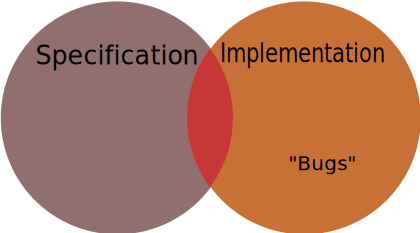
\includegraphics[width=2.5in]{BuggyImplementation.png}
        \label{fig:buggy}
        \caption{Buggy Implementation. ``Bugs'' are defined as strings part of
        the implementation which are not part of the specification.}
\end{figure*}

\begin{figure*}[!t]
    \begin{center}
        \includegraphics[width=2.5in]{IncompleteImplementation.png}
        \label{fig:incomplete}
        \caption{Incomplete Implementation. The specification describes
        a ``larger'' language than the implementation.}
    \end{center}
\end{figure*}

Regular Languages are not extremely powerful, but some very useful tools,
such as grep, leverage Regular Languages through their string representation
\emph{regular expressions}. 
%TODO define Regular expressions here

Another useful property of regular
languages is, regular languages are closed under the standard set operations: union,
intersection, complement \cite[p.~45]{Sipser}.  We are now free to manipulate
our problem with standard set theory operations, and know we remain within the
context of regular languages.  
%copy closure theorum here

Our system will consume 2 programs, to determine if the
specification matches an implementation as in Figure \ref{fig:correct}.
Equation \ref{eq:basis} defines how we intend to accomplish this. 
\begin{equation}
L( M ) = L( A ) \cap \overline{L ( S ) } 
\label{eq:basis}
\end{equation}

We simply then need to analyse L(M) to determine if our implementation matches
our specification. L(M) results 2 possibilities as equation \ref{eq:lmcases}
shows.
\begin{equation}
    L(M) = 
    \begin{cases}
        \emptyset \text{ if } L(A) \equiv L(S)\\
        \text{not empty if } L(A) \subset L(S) 
    \end{cases}
    \label{eq:lmcases}
\end{equation}

Intuitively this makes sense.  If a program has ``bugs'' then the language the
implementation describes is not fully contained by the specification.  This results
in something akin to Figure \ref{fig:buggy}, furthermore its possible that the
implementation is fully contained by the specification, but the implementation
is still incomplete as in Figure \ref{fig:incomplete}.  Our Model checker simply
needs to accept 2 DFAs, and apply Equation \ref{eq:basis}.  If the result is an
empty language as in Equation \ref{eq:lmcases}, we know that the implementation
completely describes the specification.

\section{Model-Checker in C++}
The first step toward realizing an our verifier is to encode the mathematical
models into a representation which can be manipulated by the computer. This
process of encoding is best facilitated by the Ballmer Peak \cite{ballmer-peak}. 
Once we have a representable model, we can implement the required operations.
Firstly we have to convert the NFA representation to a DFA, then apply Equation
\ref{eq:basis}. Lastly, we run a search algorithm over the resultant DFA to
determine if the language is empty.

\subsection{DFA Representation}
The STL (Standard Template Library), offers 3 data structures which are
pertinent to representing the DFA: set, map, and multimap.  

\subsection{Parallel Simulation of 2 DFAs}

\subsection{The Subset Construction}
Not part of the finished implementation.

\subsection{Complexity}
Like, things get complex, and like some guy name Big-O comes and does something
about it. 
\appendices

\bibliographystyle{IEEEtran}
\bibliography{IEEEabrv,WrightSources}

\end{document}

